\documentclass[10pt,letterpaper]{article}

\usepackage[margin=1in]{geometry}
\usepackage{times}
\usepackage{amsmath}
\usepackage{amssymb}
\usepackage{graphicx}
\usepackage{tikz}
\usepackage{listings}
\usepackage{hyperref}
\usepackage{fancyhdr}

\pagestyle{fancy}
\fancyhf{}
\fancyfoot[C]{\thepage}
\renewcommand{\headrulewidth}{0pt}

\setlength{\parindent}{0pt}
\setlength{\parskip}{10pt}

\lstset{
    basicstyle=\ttfamily\small,
    frame=none,
    numbers=none,
    breaklines=true
}

\begin{document}

\begin{center}
{\Large\bfseries Montana: Finality from Sequential Computation}

\vspace{18pt}

Alejandro Montana\\
github.com/afgrouptime\\
x.com/tojesatoshi

\end{center}

\vspace{12pt}

\textbf{Abstract.}  A purely self-sovereign finality mechanism would allow distributed systems to achieve irreversible consensus without economic security or honest majority assumptions.  Verifiable Delay Functions provide part of the solution, but the main benefits are lost if finality still depends on external validators or stake.  We propose a solution to the finality problem using accumulated VDF checkpoints.  The system chains sequential computations by hashing each checkpoint into the next, forming a record that cannot be changed without redoing the sequential work.  The deepest VDF chain not only serves as proof of elapsed time, but proof that equivalent wallclock time was expended.  As long as physics holds, attackers cannot rewrite N checkpoints faster than N × T seconds regardless of computational resources.  The system requires minimal structure and no external dependencies.

\section{Introduction}

Distributed systems have come to rely on external mechanisms to achieve finality.  Proof-of-work systems provide probabilistic finality through computational races.  Proof-of-stake systems provide economic finality through slashing conditions.  Byzantine fault tolerant systems provide deterministic finality through supermajority votes.

The problem of course is that all these mechanisms require trust in collective behavior.  Miners must be trusted not to reorg.  Validators must be trusted not to collude.  Supermajorities must be trusted to remain honest.  The cost of violating finality is economic or probabilistic, not physical.

What is needed is a finality mechanism based on physical constraints instead of trust, allowing any node to verify finality independently without relying on external parties.  Computations that are physically impossible to accelerate would protect against rewriting history, and the cost of attack would be time itself.

In this paper, we propose a solution to the finality problem using accumulated Verifiable Delay Function checkpoints.  The system is secure as long as VDF sequentiality holds and adversaries operate within known physics.

\section{Temporal Time Unit}

We define a Temporal Time Unit as a cryptographic proof of elapsed time.  The unit asymptotically approaches one second as verification evidence accumulates:

\begin{equation}
\lim_{\text{evidence} \to \infty} 1\text{ }\text{\TH} \to 1\text{ second}
\end{equation}

Each owner transfers units by digitally signing a hash of the previous transaction and the public key of the next owner.  A recipient can verify the signatures to verify the chain of ownership.

The problem of course is the recipient cannot verify that time actually passed.  A common solution is to introduce a trusted timestamp authority, but this returns to the trust model.  We need a way for any node to verify elapsed time without trusting a central party.

\section{VDF Checkpoint}

The solution we propose begins with a Verifiable Delay Function.  A VDF works by computing T sequential hash iterations that cannot be parallelized:

\begin{equation}
\text{VDF}(x, T) = H^T(x) = \underbrace{H(H(H(...H(x)...)))}_{T \text{ iterations}}
\end{equation}

The VDF proves that minimum time T has elapsed.  Each checkpoint includes the previous checkpoint in its input, forming a chain:

\begin{center}
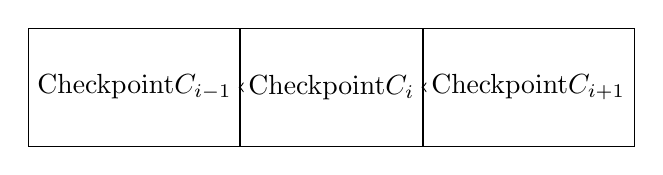
\begin{tikzpicture}[node distance=2.5cm]
\tikzstyle{block} = [rectangle, draw, minimum width=2cm, minimum height=1.5cm]
\node[block] (b1) {Checkpoint\\$C_{i-1}$};
\node[block, right of=b1] (b2) {Checkpoint\\$C_i$};
\node[block, right of=b2] (b3) {Checkpoint\\$C_{i+1}$};
\draw[->] (b1) -- (b2);
\draw[->] (b2) -- (b3);
\end{tikzpicture}
\end{center}

\begin{equation}
C_i = \text{VDF}(C_{i-1} \| B_i, T)
\end{equation}

Where $T = 2^{24}$ iterations of SHAKE256, approximately 2.5 seconds.

\section{Accumulated Finality}

To accomplish finality without external trust, we accumulate VDF checkpoints.  Each checkpoint requires T sequential computation.  Reverting N checkpoints requires N × T sequential computation.

\begin{center}
\begin{tabular}{|l|l|l|}
\hline
\textbf{Depth} & \textbf{Checkpoints} & \textbf{Attack Cost} \\
\hline
Soft & 1 & 2.5 seconds \\
Medium & 100 & 4 minutes \\
Hard & 1000 & 40 minutes \\
\hline
\end{tabular}
\end{center}

An adversary with unbounded parallelism still needs N × 2.5 seconds of wallclock time to rewrite N checkpoints.  This follows from VDF sequentiality—the same property that makes VDFs useful for randomness beacons.

The probability of an attacker catching up diminishes not exponentially with hashpower, but linearly with time deficit.  There is no lucky catch-up.  Time cannot be parallelized.

\section{Network}

The steps to run the network are as follows:

\begin{enumerate}
\item New transactions are broadcast to all nodes.
\item Full nodes collect transactions and compute VDF checkpoints.
\item Each checkpoint chains to the previous, proving elapsed time.
\item Nodes accept the deepest valid VDF chain as canonical.
\item Light nodes verify checkpoint proofs without computing VDFs.
\end{enumerate}

Nodes always consider the deepest VDF chain to be correct.  If two nodes broadcast different checkpoints simultaneously, nodes work on the first received.  The tie breaks when the next VDF completes—whichever chain extends first becomes deeper.

New checkpoint broadcasts do not need to reach all nodes instantly.  As long as they propagate before the next VDF period, the network maintains consistency.

\section{Incentive}

By convention, the first transaction in a block distributes new Temporal Time Units to participants.  This provides incentive for nodes to support the network and distributes units into circulation without a central issuer.

The distribution follows a halving schedule:

\begin{center}
\begin{tabular}{|l|l|l|}
\hline
\textbf{Era} & \textbf{Per Block} & \textbf{Cumulative} \\
\hline
1 & 3,000 \TH\ (50 min) & 50\% \\
2 & 1,500 \TH\ (25 min) & 75\% \\
3 & 750 \TH\ (12.5 min) & 87.5\% \\
... & ... & ... \\
33 & 1 \TH\ (1 sec) & 100\% \\
\hline
\end{tabular}
\end{center}

Total supply: 1,260,000,000 \TH\ = 21,000,000 minutes.

Pre-allocation: 0.

\section{Time Verification}

The system verifies elapsed time through two mechanisms:

\textbf{Atomic Time Consensus.}  34 NTP servers across 8 geographic regions provide time reference.  Consensus requires >50\% agreement within 1 second.  This is engineering, not security—the VDF enforces minimum elapsed time regardless of reported clock values.

\textbf{VDF Proof.}  Each checkpoint proves T sequential iterations occurred.  The construction uses iterated hashing—simpler than group-based VDFs (Wesolowski, Pietrzak) but with the same sequentiality property.  Verification uses STARK proofs for O(log T) complexity.  The VDF cannot be accelerated regardless of parallel resources.

\section{Privacy}

The necessity to announce all transactions publicly precludes traditional privacy, but privacy can be maintained by keeping public keys pseudonymous.  The public sees that someone transfers an amount to someone else, but without information linking the transaction to anyone.

As an additional measure, a new key pair should be used for each transaction.  Some linking is unavoidable with multi-input transactions, which reveal that inputs belong to the same owner.

Optional privacy tiers provide additional protection:

\begin{center}
\begin{tabular}{|l|l|}
\hline
\textbf{Tier} & \textbf{Visibility} \\
\hline
T0 & Transparent \\
T1 & Hidden recipient \\
T2 & Hidden amount \\
T3 & Full privacy \\
\hline
\end{tabular}
\end{center}

\section{Calculations}

We consider the scenario of an attacker trying to rewrite history.  Unlike probabilistic systems, the attacker cannot get lucky.  Rewriting N checkpoints requires exactly N × T sequential computation.

Let $d$ = attacker's time deficit in checkpoints.  The time required to catch up:

\begin{equation}
t_{\text{catch-up}} = d \times T
\end{equation}

During this time, honest nodes extend the chain by:

\begin{equation}
n_{\text{honest}} = \frac{t_{\text{catch-up}}}{T} = d
\end{equation}

The attacker never catches up.  The deficit remains constant or grows.

\begin{lstlisting}
#include <math.h>

double TimeToRewrite(int checkpoints, double vdf_time)
{
    return checkpoints * vdf_time;
}

// Example: rewriting 1000 checkpoints
// TimeToRewrite(1000, 2.5) = 2500 seconds = 41.7 minutes
\end{lstlisting}

Results for various depths:

\begin{verbatim}
checkpoints=1      time=2.5 seconds
checkpoints=10     time=25 seconds
checkpoints=100    time=4.2 minutes
checkpoints=1000   time=41.7 minutes
checkpoints=10000  time=6.9 hours
\end{verbatim}

\section{Post-Quantum Security}

The system uses post-quantum cryptographic primitives:

\begin{center}
\begin{tabular}{|l|l|l|}
\hline
\textbf{Function} & \textbf{Primitive} & \textbf{Standard} \\
\hline
Signatures & SPHINCS+-SHAKE-128f & NIST FIPS 205 \\
Key Exchange & ML-KEM-768 & NIST FIPS 203 \\
Hashing & SHA3-256, SHAKE256 & NIST FIPS 202 \\
VDF & Iterated SHAKE256 & — \\
\hline
\end{tabular}
\end{center}

The VDF construction uses hash iteration, which remains secure against quantum computers.  Grover's algorithm provides at most quadratic speedup for search, but does not break sequential iteration.

\section{Assumptions}

The security model rests on explicit assumptions:

\begin{enumerate}
\item \textbf{VDF Sequentiality.}  No algorithm computes $H^T(x)$ faster than T sequential evaluations.  If broken, finality degrades to the broken primitive's security.  T is fixed at $2^{24}$: specialized hardware may provide constant-factor speedup (bounded by circuit physics), but not asymptotic improvement.  The system degrades gracefully—2x faster hardware halves attack cost, but attack cost remains non-zero time.

\item \textbf{Hash Integrity.}  SHAKE256 has no structural weakness enabling iteration shortcuts.  If broken, same degradation.

\item \textbf{Physical Bounds.}  Adversaries operate within known physics.  Cannot reverse causality, signal faster than light, or compute without energy.  If broken, all cryptography fails.
\end{enumerate}

\section{Conclusion}

We have proposed a system for finality without relying on economic security or honest majority.  We started with the framework of Verifiable Delay Functions, which provide sequential computation guarantees, but are incomplete without a way to accumulate finality.  To solve this, we proposed chaining VDF checkpoints such that reverting N of them requires N × T wallclock time.

The system provides finality bounded by physics.  Nodes verify independently by checking the VDF chain.  No validators to query, no stake to count, no attestations to trust.  The proof is the computation itself.

As long as VDF sequentiality holds and adversaries operate within known physics, the accumulated VDF chain provides finality that cannot be reversed without expending equivalent time.

\section*{References}

\begin{enumerate}
\item D. Boneh, J. Bonneau, B. Bünz, B. Fisch, "Verifiable Delay Functions," CRYPTO 2018.
\item NIST FIPS 202, "SHA-3 Standard," 2015.
\item NIST FIPS 203, "Module-Lattice-Based Key-Encapsulation Mechanism," 2024.
\item NIST FIPS 205, "Stateless Hash-Based Digital Signature Standard," 2024.
\item L. Lamport, "Time, Clocks, and the Ordering of Events," 1978.
\item Y. Sompolinsky, A. Zohar, "PHANTOM," 2018.
\item S. Haber, W.S. Stornetta, "How to Time-Stamp a Digital Document," 1991.
\end{enumerate}

\end{document}
